\chapter[Introduction]{Introduction}
\vspace{12pt}

\vspace{12pt}

  
The popularity of mobile broadband has grown rapidly in recent years. Report from the International Telecommunication Union \cite{no_of_mobile_devices_ICTFacts} has shown that in 2015 alone there are more
than 7 billion mobile cellular subscriptions, corresponding to a penetration rate of 97\%,
up from 738 million in 2000. And it also states that globally, mobile broadband penetration
reaches 47\% in 2015, a value that increased 12 times since 2007. And the competitive nature of the mobile phone market has pushed manufacturers to manufacture and innovate in a rapid phase. This means consumers can buy highly sophisticated devices for very cheaper prices.

\vspace{12pt}

Nowadays mobile devices have multiple interfaces with different characteristics for their communication. These interfaces can be infrastructure networks like cellular or infrastructure-less networks like   WIFI  -Direct or Bluetooth. The availability of these vastly different network interfaces and communication protocols in mobile devices has open new research opportunities in providing reliable, low-cost, high bandwidth connections without any additional cost.

\vspace{12pt}

With mobile devices, Internet traffic surpassing that of computers the need for a reliable, low-cost high bandwidth mobile connection is apparent more than ever. Cisco Visual Networking Index: Global Mobile Data Traffic Forecast Update, 2017–2022\cite{mobile_web_penetration}. In the past, this problem has been addressed by implementing ad-hoc networks. This is a good solution as we have a high density of mobile devices in most of the crowded place. But the thing about the ad-hoc network is that they can be very unpredictable. As ad-hoc infrastructure-less in nature   WIFI   and Bluetooth connections are better suited than their cellular counterpart. The use of Bluetooth connection is not ignored due to the low bandwidth connections they make.

\vspace{12pt}

In the past researchers have tried to solve this problem by implementing an ad-hoc network using only the   WIFI   interface.  To my knowledge, the most important part of an ad-hoc network is to keep track of information about the nodes in real-time. In the past researchers have used a separate channel in the ad-hoc network for this.(Liu, et al.2016)\cite{GO}. Due to the ad-hoc network being unreliable this is not a good solution.

\vspace{12pt}

These days the mobile devices have become very sophisticated. They possess multiple network interfaces with considerable processing power. Technologies like GSM and   WIFI   had become matured technologies. Nowadays GSM networks can provide good coverage in a very reliable manner. GSMA - Network Coverage statistics \cite{GSMANetwork_coverage}. With the introduction of  WIFI  p2p technologies like  WIFI-Direct, it has become very easy to form a peer to peer networks using  WIFI  interfaces. So this shift of paradigm provides a unique research opportunity in developing a hybrid network that uses  WIFI  peer to peer networks as its data plane and cellular network as its control plane and the backup data plane.

\vspace{12pt}

The proposed architecture has two network interfaces working in a multiplexing manner to provide network connections. Every device consists of a demon(a simple program that keeps track of the node state in real-time) that calls to a server giving metadata about the node. It processes those data and comes up with routing paths for the ad-hoc network. Then the server transfers back the relevant data for the available nodes to provide an optimized routing path. So when we need to transfer data to a device in the ad-hoc network it uses  WIFI  p2p rather than cellular saving the valuable bandwidth. Traffic that is gong to the Internet is routed to the GSM network using the cellular interface without any change.

\vspace{12pt}

 Generally,  WIFI  networks have greater bandwidth than that of a GSM network. So it is evident that we can improve the speed if we use  WIFI  connection rather than a cellular connection. As we are using a much reliable GSM network for our control plane can provide a stable connection than a pure ad-hoc network. The usage of local routing in the ad-hoc network can provide a cheap reliable high bandwidth low latency connection in some scenarios. We are going to investigate the efficiency of this with the previous Android  MANET implementation and current GSM connections to further justify the significance of this solution. 

\vspace{12pt}
\clearpage



\section{Motivation}



\vspace{12pt}

According to the Telecommunication Development Bureau of ITU statistics \cite{no_of_mobile_devices_ICTFacts} by the end of 2015, there are more than 7 billion active mobile cellular subscriptions worldwide. According to them globally, mobile broadband penetration reaches 47\% in 2015, a value that increased 12 times since 2007. So it is obvious that mobile broadband is a dynamic market segment. 

\vspace{12pt}


Telecommunication Development Bureau of ITU estimates that the 3G coverage has increased from 45\% to 69\% from 2011 to 2015. This corresponds to 29\% present 3G coverage in rural areas and 89\% in urban areas. Some developed countries like the USA have higher mobile broadband penetration at around 78\% while some developing countries like Africa have a mobile broadband penetration around 17.4\% So with the above statistical evidence, we can say that mobile broadband penetration needs to improve in most parts of the world.

\vspace{12pt}


With the emergence of web 2.0, most of the popular application has become web-based ones. The majority of current applications nowadays need a working Internet connection to function properly.  According to the Cisco VNI Mobile\cite{mobile_web_penetration}, there is a significant increase in mobile traffic for the past few years and it is expected to grow at a rapid phase. They further point out that the share of smart devices and connections as a percentage of the total will increase from 53 per cent in 2017 to nearly three-fourths, at 73 per cent, by 2022. So with the above evidence, it is safe to say there is a shift of paradigm for Internet    traffic from personal computers to mobile devices 

\vspace{12pt}


According to the above source\cite{mobile_web_penetration}, the majority of users are shifting from static web content to dynamic web content in recent years. These dynamic content can vary from video streaming applications to multiplayer virtual reality games. As they are dynamic they need very high bandwidth, low latency connection to function properly.

\vspace{12pt}


As they point out in Facts and Figures 2019 by the Telecommunication Development Bureau of ITU\cite{no_of_mobile_devices_ICTFacts} the cost of data for mobile devices has not become sufficiently cheap when comparing to that of the developing countries. According to them only developed countries and some of the developing countries can achieve the relevant pricing for broadband data in the world. 


\vspace{12pt}
\clearpage


In recent years mobile devices have become sophisticate in various aspects. Mobile processors have gained in processing power while increasing power efficiency. This is evident when comparing the benchmark of those old ones with new ones. The charge capacity of current mobile devices batteries has gained many improvements in recent years. The majority of mobile devices have at least one-day battery life. They

\vspace{12pt}


Currently, almost all of the smartphones possess multiple network interfaces for communication. They can be of Cellular interfaces in which devices can support different protocols and multiple network bands or  WIFI  interfaces with dual-band support built. These networks have a rich diversity of properties unique to them. For example, cellular networks are reliable, high-cost, long-range with limited bandwidth connections while Ad-hoc networks have volatile, short-range and high-bandwidth connections. If somehow we can make a hybrid network using the best qualities of each interface then we can improve the quality of the network for a vast number of mobile broadband users.

\vspace{12pt}


In the past approach for this kind of problem is to make a mobile ad-hoc network using the  WIFI  interface of the devices. COMONet(Wijesekera and Keppitiyagama 2007)\cite{comonet}. In the past, cellular technology has not matured to use it side by side with  WIFI  ad-hoc network. As we are approaching the problem in the present time a lot of scenarios have changed for the better. With the emergence of the Android open source project, it has become easy to work with the inner working of the mobile devices. In the past major mobile OS source codes were not publicly available. So to get an idea of the inner working of the device OS researcher needs to read the OS binary files using special kind of software and reverse engineer a solution \cite{comonet}. modification  Due to Android  OS, using Linux as its kernel network modification to Android devices has become much more feasible than before.
 
\vspace{12pt}


So with these changes, most of the old limitations in solving such a problem are no more. So as a computer science student, it is evident that we need to revisit the problem. We need to use these newfound opportunities to provide a better solution in solving this apparent communication need. If we can provide such a solution it will become a widely impactful one. 

\vspace{12pt}
\clearpage



\section{Research significance}
\vspace{12pt}
Most of the mobile devices in the present era needs Internet access to properly function. But the current offering from the cellular broadband providers is not on par with this demand. In the past, this kind of problem needs to be addressed using peer to peer Ad hoc networks. To create the ad hoc network researchers use a single network interface to implement the peer to peer network. Even though that was the best solution at that time it is not the case in the present. What this researcher is proposing is a hybrid between the cellular and  WIFI  peer to peer networks that uses the cellular network as its control plane and the backup connection while using the  WIFI  p2p connection as the main data channel.

\vspace{12pt}
With the emergence of new paradigms like AR and VR applications, online games, people need high-quality network connections for a cheap price to get most out of these applications. For example, let’s consider the new AR multiplayer games. Those need low latency, high bandwidth connection between the local devices to function properly. Those applications need the Internet connection side by side to function. For this kind of application, this is an ideal solution. This will be a great addition to creating a local connection that needs more than the bandwidth provided by the general Bluetooth connections. Examples for this kind of apps can be varying from Video editing studios that can multiplex different video streams run on Android devices, Classroom teaching applications, AR, VR applications, Multiplayer games to Local peer to peer chat applications.

\vspace{12pt}
As this network can be implemented using already available hardware in the mobile systems there is no additional cost involved. Networking Protocols we use are already implemented in the Android OS and Linux kernel. The only drastic modification we are doing is to use root access to change the routing tables in the devices. If this can be implemented using the OS level we can mitigate this limitation as well.

\vspace{12pt}
As for the contribution to the Computer Science community, there is no implementation of this kind of network in the current time. So this research opens the door to a new frontier of technology. As this research is implementing a working prototype of the proposed network the researcher can see what kind of problems are there. Most of the previous implementations did not use cellular side by side due to its being less matured nature. But now it is a fully matured system in most of the areas of the world. So by revisiting the old problem, the researcher can understand the current problems that need to address in such a network. 

\vspace{12pt}
In the past, node discovery has not been done in an automated manner. This research addresses that particular problem. This itself is a massive problem as the control plane needs to keep track of the node metadata in real-time. Control planes operating on cellular connections efficiently address this problem. This is a great milestone in the hybrid mesh networking paradigm. 

\vspace{12pt}
The gains from the current hybrid network for the current smartphone users is a huge one. They will get a more reliable network with higher local bandwidth and lower latency for a cheaper price. This will create the opportunity for different categories of applications that rely on high local bandwidth connection as this connection is free compared to cellular ones.



\vspace{12pt}

\section{Related Technologies}
\vspace{12pt}


\vspace{12pt}


\subsection{What are wireless Networks}
\vspace{12pt}

A wireless network is a computer network that uses wireless data connections between network nodes. They are very useful in scenarios where it is either costly or impractical to use wires to connect the nodes in the networks. They are particularly useful for connecting mobile nodes to a network. They use different ranges of the electromagnetic spectrum to make wireless links between network nodes.

\vspace{12pt}

In general, when we increase the frequency of the electromagnetic spectrum in the data link we will have higher bandwidth. At the same time, this will decrease the rage of the datalink needing more nodes to cover the same area. On the other side if we use low frequency in the electromagnetic spectrum for the data link it will increase the range of the network while decreasing the bandwidth of the connection.

\vspace{12pt}

There are various kinds of wireless networks that are currently in use. Those can be currently categorized as fallows. 


\vspace{12pt}
\clearpage
\subsubsection{Wireless personal area Network(PAN)}


\vspace{12pt}

 These are used in connecting devices within a relatively small area, that is generally within a person's reach. Generally, they are low power, low bandwidth connections which used to connect personal devices. Bluetooth, ZigBee networks are examples of this kind of network.

 \vspace{12pt}
 
  \subsubsection*{wireless local area Network (WLAN)}
  \vspace{12pt}
  wireless local area network (WLAN) links two or more devices over a short distance using a wireless distribution method. It usually provides a connection through an access point for Internet access. 
  
  \vspace{12pt}
  
  The use of spread-spectrum or orthogonal frequency-division multiplexing(OFDM) technologies may allow users to move around within a local coverage area and remain connected to the network. There can be fixed wireless technology that implements point-to-point links between computers or networks at two distant locations, often using the dedicated microwave or modulated laser light beams over the line of sight.
  
    \vspace{12pt}
    
 WIFI  network connections belong to this category of networks. Any device that uses the IEEE 802.11 WLAN standards are marketed under the Wi-Fi brand name.

 \vspace{12pt}





 \subsubsection*{Wireless Ad-Hoc Network}
  \vspace{12pt}
 A wireless ad hoc network, also known as a wireless mesh network or mobile ad hoc network (MANET), is a wireless network made up of radio nodes organized in a mesh topology. Each node forwards messages on behalf of the other nodes and each node perform routing. Ad hoc networks can "self-heal", automatically re-routing around a node that has lost power
 

 \vspace{12pt}





 \subsubsection*{Wireless wide area Networks(WAN)}
  \vspace{12pt}
 
 These networks can be used to connect distance nodes using directional antennas on the 2.4 GHz and 5.8Ghz frequency bands of the electromagnetic spectrum. we are not using this kind of networks in our research currently. 

 \vspace{12pt}


\subsection{Cellular Networks}

\vspace{12pt}

The major different of this network is that the network is distributed over land areas called "cells", each served by at least one fixed-location transceiver, but more normally, three cell sites or base transceiver stations. These base stations provide the cell with the network coverage which can be used for transmission of voice, data, and other types of content. A cell typically uses a different set of frequencies from neighbouring cells, to avoid interference and provide guaranteed service quality within each cell.\cite{patent}

\vspace{12pt}


When joined together, these cells provide radio coverage over a wide geographic area. This enables numerous portable transceivers (e.g., mobile phones, tablets, and laptops equipped with mobile broadband modems, pagers, etc.) to communicate with each other and with fixed transceivers and telephones anywhere in the network, via base stations, even if some of the transceivers are moving through more than one cell during transmission.


\vspace{12pt}

In cities, each cell site may have a range of up to approximately 1⁄2 mile (0.80 km), while in rural areas, the range could be as much as 5 miles (8.0 km). It is possible that in clear open areas, a user may receive signals from a cell site 25 miles (40 km) away.

\vspace{12pt}
There are several different digital cellular technologies, including Global System for Mobile Communications (GSM), General Packet Radio Service (GPRS), CDMA One, CDMA2000, Enhanced Data Rates for GSM Evolution (EDGE), Universal Mobile Telecommunications System (UMTS). Further details on those technologies are out of the scope of this research so it will be pointless to describe those here.

\vspace{12pt}

Cellular networks offer several desirable features:

\vspace{12pt}

\begin{itemize}
  \item More capacity than a single large transmitter, since the same frequency can be used for multiple links as long as they are in different cells.
  \item Mobile devices use less power than with a single transmitter or satellite since the cell towers are closer
  \item Larger coverage area than a single terrestrial transmitter, since additional cell towers can be added indefinitely and are not limited by the horizon.
  \item Reliability of the network as it uses multiple node connections at the same time.
\end{itemize}

\vspace{12pt}
Currently, there are different generations of networks varying from the first generation networks to the fifth generation of networks for mobile phones. Currently, 3G and 4G networks are widely used worldwide for mobile broadband connections. 5G networks are currently at its early adoption stage  As we are using those technologies lets consider those technologies in detail.
\vspace{12pt}

\subsubsection{What are 3G Networks}
\vspace{12pt}

3G is the third generation of wireless mobile telecommunications technology. It is the upgrade for 2G and 2.5G GPRS networks, for faster data transfer speed. This is based on a set of standards used for mobile devices and mobile telecommunications use services and networks that comply with the International Mobile Telecommunications -2000 (IMT-2000) specifications by the International Telecommunication Union.

\vspace{12pt}
3G telecommunication networks support services that provide an information transfer rate of at least 144 kbit/s.\cite{d_speed} Later 3G releases often denoted 3.5G and 3.75G, also provide mobile broadband access of several Mbit/s to smartphones and mobile modems in laptop computers. This ensures it can be applied to wireless voice telephony, mobile Internet access, fixed wireless Internet access, video calls, and mobile TV technologies.


\vspace{12pt}
it is expected that IMT-2000 will provide transmission rates: a minimum data rate of 2 Mbit/s for stationary or walking users, and 348 kbit/s in a moving vehicle," and this can be varied from a different carrier to carrier. \cite{about_mobi}





\vspace{12pt}

\subsubsection{What are 4G Networks}
\vspace{12pt}

This as a communication standard set by the International Telecommunications Union-Radio communications sector (ITU-R). They specified a set of requirements for 4G standards, named the International Mobile Telecommunications Advanced (IMT-Advanced) specification, setting peak speed requirements for 4G service at 100 megabits per second (Mbit/s)(=12.5 megabytes per second) for high mobility communication (such as from trains and cars) and 1 gigabit per second (Gbit/s) for low mobility communication (such as pedestrians and stationary users)\cite{Requirement}


\vspace{12pt}
\clearpage
This standard is implemented using different IMT-2000 compliant 4G standards such as LTE Advanced, 3GPP Long Term Evolution (LTE), Mobile WiMAX (IEEE 802.16e). Currently, this is being replaced by a 5G standard.


\vspace{12pt}



\subsubsection{What are 5G Networks}
\vspace{12pt}
5G is the fifth-generation wireless technology for digital cellular networks that have begun wide deployment in 2019. Like previous standards, the covered areas are divided into regions called cells, serviced by individual antennas. The frequency spectrum of 5G is divided into millimetre waves, mid-band, and low-band. Low-band uses a similar frequency range as the predecessor.


\vspace{12pt}
Initially, the term was associated with the International Telecommunication Union's IMT-2020 standard, which required a theoretical peak download speed of 20 gigabits per second and 10 gigabits per second upload speed, along with other requirements. But the actual speeds can be ranged from 50 Mbit/s to over a gigabit. Mid-band 5G, by far the most common, will usually deliver between 100 to 400 Mbit/s.

\vspace{12pt}


Frequencies are above 24 GHz reaching up to 72 GHz which is above Extremely high frequency's lower boundary. The reach of these antennas is short, so more cells are required. Millimetre waves have difficulty traversing many walls and windows, so indoor coverage is limited.

\vspace{12pt}

Currently, there is no 5G coverage in Sri Lanka when conducting this research. SO we cannot practically say anything about this technology. But due to the limited coverage of these 5G networks need for a hybrid network to mitigate the downsides will become apparent more than ever.

\vspace{12pt}
\clearpage
\subsection{What are WIFI Networks}


\vspace{12pt}

Wi-Fi is a family of wireless networking technologies, based on the IEEE 802.11 family of standards, which are commonly used for local area networking of devices and Internet access. 

\vspace{12pt}

Wi-Fi uses multiple parts of the IEEE 802 protocol family and is designed to seamlessly work with Ethernet. The data is organized into 802.11 frames that are very similar to Ethernet frames at the data link layer, but with extra address fields. MAC addresses are used as network addresses for routing over the LAN. Compatible devices can network through a wireless access point to each other as well as to wired devices and the Internet. The different versions of Wi-Fi are specified by various IEEE 802.11 protocol standards, with the different radio technologies determining radio bands, and the maximum ranges, and speeds that may be achieved. 


\vspace{12pt}


Wi-Fi most commonly uses the 2.4 gigahertz (120 mm) UHF and 5 gigahertz (60 mm) SHF ISM radio bands. Most of the current devices can use both of these bands simultaneously. These bands are subdivided into multiple channels. Channels can be shared between networks but only one transmitter can locally transmit on a channel at any moment in time.


\vspace{12pt}


Wi-Fi's wavebands have relatively high absorption and work best for line-of-sight use. Many common obstructions such as walls, pillars, home appliances, etc may greatly reduce range, but this also minimizes interference between different networks. An access point (or hotspot) often has a range of about 20 meters (66 feet) indoors while some modern access points claim up to a 150-meter (490-foot) range outdoors. 

\vspace{12pt}

Hotspot coverage can be as small as a single room with walls that block radio waves, or as large as many square kilometres using many overlapping access points with roaming permitted between them. Over time the speed and spectral efficiency of Wi-Fi have increased. As of 2019, at close range, some versions of Wi-Fi running on suitable hardware can achieve speeds of over 1 Gbit/s (gigabit per second).


\vspace{12pt}

Equipment frequently supports multiple versions of Wi-Fi but to communicate two devices must use a common Wi-Fi version. The versions differ between the radio wavebands they operate on, the radio bandwidth they occupy, the maximum data rates they can support and other details. Some versions permit the use of multiple antennas, which permits greater speeds as well as reduced interference. Fallow is a table explaining those different standards.

\vspace{12pt}

\begin{table}
\centering
\begin{tabular}{| c | c | c | c |}
\hline
IEEE Standard & Maximum link rate & Adopted & Frequency \\
\hline
 802.11b & 1 to 11 Mbit/s & 1999 & 2.4 GHz\\ 
 \hline 
 802.11a & 1.5 to 54 Mbit/s & 1999 & 5 GHz\\
 \hline   
  802.11g & 3–54 Mbit/s & 2003 & 2.4 GHz\\
 \hline
  Wi‑Fi 4 & 72–600 Mbit/s & 2009  &	2.4/5 GHz \\
 \hline
  Wi‑Fi 5 & 433–6933 Mbit/s & 2014 & 	5 GHz \\
 \hline
  Wi‑Fi 6 & 600–9608 Mbit/s & 2019	& 2.4/5 GHz \\
 \hline  
\end{tabular}
\caption{Theoretical Bandwidths of different  WIFI  standards}
\label{table1}

\end{table}



\vspace{12pt}

 WIFI  networks can function in different network modes. They are Infrastructure mode, Ad hoc mode and  WIFI  -direct mode.

\vspace{12pt}
\subsubsection{Infrastructure mode}


\vspace{12pt}

In infrastructure mode, which is the most common mode used, all communications go through a base station. For communications within the network, this introduces an extra use of the airwaves but has the advantage that any two stations that can communicate with the base station can also communicate through the base station, which enormously simplifies the protocols.

\vspace{12pt}

\subsubsection{Ad-Hoc mode}


\vspace{12pt}
According to Toh, C. (2002). Ad hoc wireless networks: Protocols and systems. \cite{book_adhoc} an ad hoc network is a network that is comprised of individual devices interacting with each other directly. The term(ad-hoc) implies spontaneous or impromptu construction because these networks often bypass the central access point such as a router.

\vspace{12pt}

Many ad hoc networks are local area networks where devices are enabled to send data directly to one another rather than going through a centralized access point. In more complex protocols nodes may forward packets, and nodes keep track of how to reach other nodes, even if they move around.

\clearpage
\vspace{12pt}

Ad-hoc mode was first invented and realized by Chai Keong Toh in his 1996 invention\cite{book} of Wi-Fi ad-hoc routing, implemented on Lucent WaveLAN 802.11a wireless on IBM ThinkPads over a size nodes scenario spanning a region of over a mile. The success was recorded in Mobile Computing magazine (1999)\cite{book}  and later published formally in IEEE Transactions on Wireless Communications, 2002\cite{book}  and ACM SIGMETRICS Performance Evaluation Review, 2001.\cite{book}.

\vspace{12pt}
This wireless ad hoc network mode has proven popular with multiplayer handheld game consoles, such as the Nintendo DS, PlayStation Portable, digital cameras, and other consumer electronics devices.
\vspace{12pt}

\subsubsection{WIFI Direct mode}


\vspace{12pt}

According to Wi-Fi Alliance(2019, Aug) www.wi-fi.org/discover-wi-fi/wi-fi-direct \cite{WiFiDirect-by-wifi-aliance}, Wi-Fi Direct is a Wi-Fi communication standard that facilitates device connections without requiring a wireless access point (WAP). The devices are connected using Wi-Fi, thus achieving Wi-Fi level connection and transfer speeds from the connectivity.


\vspace{12pt}

Wi-Fi Direct is single radio hop communication, not multihop wireless communication, unlike wireless ad hoc networks and mobile ad hoc networks. Wi-Fi ad hoc mode, however, supports multi-hop radio communications, with intermediate Wi-Fi nodes as packet relays.	
\vspace{12pt}

The basic function of the Wi-Fi Direct is to enable the connection between devices and facilitate data transfer through the use of built-in wireless modules without the aid of a dedicated access point.

\vspace{12pt}
Wi-Fi Direct has become a standard feature in smartphones, portable media players, and feature phones as well. The process of adding Wi-Fi to smaller devices has accelerated, and it is now possible to find printers, cameras, scanners and many other common devices with Wi-Fi in addition to other connections, like USB.
\vspace{12pt}
\clearpage
\subsubsection{Multiple access points}
\vspace{12pt}
An Extended Service Set may be formed by deploying multiple access points that are configured with the same SSID and security settings. Wi-Fi client devices typically connect to the access point that can provide the strongest signal within that service set. increasing the number of Wi-Fi access points for a network provides redundancy, better range, support for fast roaming and increased overall network-capacity by using more channels or by defining smaller cells.
\vspace{12pt}

\subsection{A Peer-to-Peer (P2P) Network}


\vspace{12pt}
According to (Schollmeier,2001)\cite{define_P_to_p}, peer-to-peer network is a network of interconnected nodes (”peers”) serving resources amongst each other without the use of a centralized administrative system. Due to not having a centralized system, the network is resilient for node failures. Peers make a portion of their resources, such as processing power, disk storage or network bandwidth, directly available to other network participants, without the need for central coordination by servers or stable hosts. Peers are both suppliers and consumers of resources, in contrast to the traditional client-server model in which the consumption and supply of resources are divided.

\vspace{12pt}
\subsubsection{Architecture}
\vspace{12pt}
A peer-to-peer network is designed around the notion of equal peer nodes simultaneously functioning as both "clients" and "servers" to the other nodes on the network. This model of network arrangement differs from the client-server model where communication is usually to and from a central server.

\vspace{12pt}

Peer-to-peer networks generally implement some form of virtual overlay network on top of the physical network topology. The nodes in the overlay form a subset of the nodes in the physical network. Data is still exchanged directly over the underlying TCP/IP network, but at the application, layer peers can communicate with each other directly, via the logical overlay links (each of which corresponds to a path through the underlying physical network). Overlays are used for indexing and peer discovery and make the P2P system independent from the physical network topology.
\vspace{12pt}
\clearpage
Based on how the nodes are linked to each other within the overlay network, and how resources are indexed and located, we can classify networks as unstructured, structured or as a hybrid between the two.
\vspace{12pt}
\begin{itemize}
	\item  Unstructured networks 
	\item   Structured networks 
	\item  Hybrid networks 
	
\end{itemize}
\subsubsection{Unstructured Networks}
\vspace{12pt}
Unstructured peer-to-peer networks do not impose a particular structure on the overlay network by design, but rather are formed by nodes that randomly form connections to each other.

\vspace{12pt}
Because there is no structure globally imposed upon them, unstructured networks are easy to build and allow for localized optimizations to different regions of the overlay. Also, because the role of all peers in the network is the same, unstructured networks are highly robust in the face of high rates of "churn.
\vspace{12pt}
The primary limitations of unstructured networks also arise from this lack of structure. In particular, when a peer wants to find the desired node in the network, the search query must be flooded through the network to find as many peers as possible that knows that particular node. Flooding causes a very high amount of signalling traffic in the network which can cause network failure.

\vspace{12pt}
\subsubsection{Structured Networks}
\vspace{12pt}
In structured peer-to-peer networks, the overlay is organized into a specific topology, and the protocol ensures that any node can efficiently search the network for a file/resource.
\vspace{12pt}
The most common type of structured P2P network implements a distributed hash table (DHT), in which a variant of consistent hashing is used to assign ownership of each file to a particular peer. This enables peers to search for resources on the network using a hash table: that is, (key, value) pairs are stored in the DHT, and any participating node can efficiently retrieve the value associated with a given key.
\vspace{12pt}
However, to route traffic efficiently through the network, nodes in a structured overlay must maintain lists of neighbours that satisfy specific criteria. This makes them less robust in volatile networks. 

\vspace{12pt}
\subsubsection{Hybrid Networks}
\vspace{12pt}
Hybrid models are a combination of peer-to-peer and client-server models. A common hybrid model is to have a central server that helps peers find each other. Spotify was an example of a hybrid model\cite{paper_compare_adhoc}. There are a variety of hybrid models, all of which make trade-offs between the centralized functionality provided by a structured client-server network and the node equality afforded by the pure peer-to-peer unstructured networks. Currently, hybrid models have better performance than either pure unstructured networks or pure structured networks because certain functions, such as searching, do require a centralized functionality but benefit from the decentralized aggregation of nodes provided by unstructured networks.

\vspace{12pt}

The decentralized nature of P2P networks increases robustness because it removes the single point of failure that can be inherent in a client-server based system. As nodes connect the demand to the system increases, at the same time total capacity of the network also increases, and the likelihood of failure decreases. If one peer on the network fails to function properly, the whole network is not compromised or damaged. 
\vspace{12pt}


\subsection{Mobile Ad-Hoc Network(MANET)}
\vspace{12pt}
MANET stands for Mobile ad-hoc Network also called a wireless ad-hoc network that usually has a routable networking environment on top of a Link Layer ad hoc network. They consist of a set of mobile nodes connected wirelessly in a self-configured, self-healing network without having a fixed infrastructure.  Nodes of this network can move freely so they can make and break the connection on the fly.\cite{TETRA}
\vspace{12pt}
Characteristics of MANET
\vspace{12pt}
\begin{itemize}
	\item  Dynamic Topologies: Network topology which is typically multihop, may change randomly and rapidly with time, it can form unidirectional or bi-directional links.
	\item   Bandwidth constrained variable capacity links: As nodes have different bandwidth the capacity of the link depending on the capacity of the lowest node.
	\item  Autonomous Behavior: Each node can act as a host and router, which shows its autonomous behaviour. 
	
	\item Energy Constrained Operation: As some or all the nodes rely on batteries or other exhaustible means for their energy. Mobile nodes are characterized with less memory, power and lightweight features.
	\item Limited Security: Wireless network is more prone to security threats. A centralized firewall is absent due to its distributed nature of the operation for security, routing and host configuration.
	\item Less Human Intervention: They require minimum human intervention to configure the network, therefore they are dynamically autonomous.


	 
	
\end{itemize}
\vspace{12pt}
\subsection{Smartphone Ad-Hoc Networks(SPANs)}
\vspace{12pt}
This is a mobile ad hoc network implementation that is done using commercially available smartphones to create peer-to-peer networks without relying on cellular carrier networks, wireless access points, or traditional network infrastructure. Apple's iPhone with version 8.4 ios and higher have been enabled with multi-peer ad hoc mesh networking capability\cite{apple}
\vspace{12pt}
\subsection{Wi-Fi Peer-to-Peer (P2P) mode in Android }
\vspace{12pt}
The Wi-Fi peer-to-peer (P2P) APIs allow applications to connect to nearby devices without needing to connect to a network or hotspot. To do this first both parties must agree to join a common network group. The connection process can be automated after that point. This function is available only for Android  devices on or above API level 14.Google (2019, Aug) Android  API documentation\cite{WiFiDirect_android}
\vspace{12pt}
This API provides a means to discover and connect to other Android devices when each device supports Wi-Fi P2P. With this API  WIFI  interface, the IP of the group owner can be found with a little effort.
\vspace{12pt}
Even though the new standard by  WIFI  -alliance includes a  WIFI  ad-hoc mode Android open-source project hasn’t implemented it. So to use the ad hoc functionality implementation of these services needs to be done. This is already done in B.A.T.M.A.N. project\cite{BATMAN} by adding ad-hoc supported kernel to Android  OS. Furthermore, this research is more focused on making a hybrid cellular ad hoc network rather than a pure ad hoc network using commercial Android devices. So implementing this kind of network is out of scope so. Furthermore, the testbed of this research consists of three Nexus 5X devices. So  WIFI  direct implementation with GO configuration is more than sufficient to simulate ad hoc property of this research.
\vspace{12pt}
\subsection{Virtual Private Network(VPN)}
\vspace{12pt}
A virtual private network (VPN) is the extension of a private network that encompasses links across shared or public networks like the Internet. VPN enables us to send data between two computers across a shared or public Internet work in a manner that emulates the properties of a point-to-point private link. (Microsoft,2019)\cite{vpn}

\vspace{12pt}
\subsection{VPN Services of Android  OS}
\vspace{12pt}
In the early days, Android  API did not have any option to perform the VPN configuration. This has to be done manually using the settings menu in the system interface. With the introduction of API Level 14, there was an option to configure the VPN using the programming API. Android  VPN service is an application interface that gives application developers to create VPN services. Google (2019, Aug) Android  API documentation https://developer.Android .com/\cite{VPNAndroid}.
\vspace{12pt}
As shown in the diagram the connection to the VPN gateway is created by the protected socket in the Android operating system. Then it creates a local tunnel interface in the Linux kernel and dumps that traffic to it. Then the traffic is channelled to and from the  Android device using virtual interfaces. Applications can access the network using those virtual interfaces.
\vspace{12pt}

\begin{figure}[H]
    \centering
   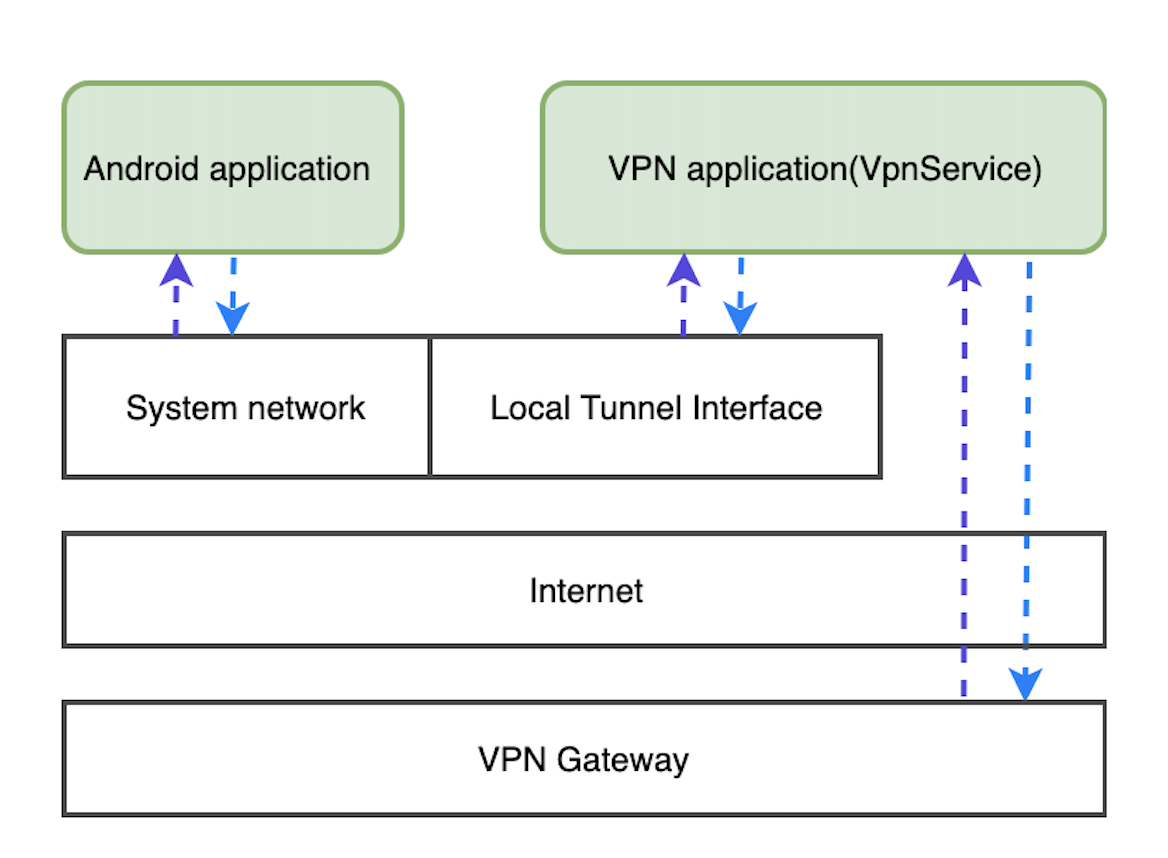
\includegraphics[scale=0.5]{images/android_vpn_api_inner_workings}
    \caption{Inner workings off the VPN implementation of Android}
    \label{fig:timeline}
\end{figure}

\vspace{12pt}
As mentioned previously the multihop ad-hoc functionality of the devices has been disabled at the OS level by restricting the creation of the interfaces by the user. But with this new VPN API, we can bypass this limitation by tunnelling the wifp2p interfaces to the tunnel interfaces. This can be illustrated as below.
\vspace{12pt}


\vspace{12pt}

\subsection{Linux kernel}
\vspace{12pt}
The Linux kernel is the main component of a Linux operating system and is the core interface between a computer’s hardware and its processes. It communicates between the two, managing resources as efficiently as possible.
\vspace{12pt}
The kernel is so named because like a seed inside a hard shell it exists within the OS and controls all the major functions of the hardware, whether it’s a phone, laptop, server, or any other kind of computer.
\vspace{12pt}
The kernel has 4 jobs:
\vspace{12pt}
\begin{itemize}
	\item Memory management: Keep track of how much memory is used to store what, and where.
	\item Process management: Determine which processes can use the CPU, when, and for how long.
	\item Device drivers: Act as mediator/interpreter between the hardware and processes.
	\item System calls and security: Receive requests for service from the processes.
\end{itemize}
\vspace{12pt}
As Linux is a monolithic kernel it includes the networking implementation already built into it. OS access the functionality of the kernel using the system call interfaces. 
\vspace{12pt}

\subsection{Ad-Hoc mode on Linux kernel}
\vspace{12pt}
Ad hoc mode has been implemented in the Linux kernel as a loadable module present in it called Kernel AODV. It implements AODV routing between computers equipped with WLAN devices.\cite{The_AODVM}
\vspace{12pt}

\subsection{Linux kernel and Android  OS}
\vspace{12pt}
According to \cite{Android_kernel} Android uses Linux kernels that are downstream of Long Term Supported (LTS) kernels and include patches of interest to the Android community that has not been merged into LTS. This means Android  Common Kernels contain additional features that are not been merged to the mainstream kernel. This can be new features tailored for Android needs (e.g. interactive cpufreq governor) to Vendor/OEM features that are useful for others (e.g. sdcardfs). Features like MPTCP, Ad-hoc routing support are not merged into Android common kernel due to not specified reasons. But as Android is open source. So anyone can add those features back and compile to get the kernel binaries.
\vspace{12pt}
\subsection{OSI layer}
\vspace{12pt}
The Open Systems Interconnection model (OSI model) is a conceptual model that characterizes and standardizes the communication functions of a telecommunication or computing system without regard to its underlying internal structure and technology. Its goal is the interoperability of diverse communication systems with standard communication protocols. The model consists of the following layers.
\vspace{12pt}
\subsubsection{Layer 1: Physical Layer}
\vspace{12pt}
The physical layer is responsible for the transmission and reception of unstructured raw data between a device and a physical transmission medium. It converts the digital bits into electrical, radio, or optical signals.
\vspace{12pt}
\subsubsection{Layer 2: Data Link Layer:}
\vspace{12pt}
The data link layer provides a node-to-node data transfer links between two directly connected nodes. It detects and possibly corrects errors that may occur in the physical layer. 
IEEE 802 divides the data link layer into two sublayers:
\cite{Overview_Architecture}
\vspace{12pt}
\begin{itemize}
	\item Medium access control (MAC) layer – responsible for controlling how devices in a network gain access to a medium and permission to transmit data.
	\item Logical link control (LLC) layer – responsible for identifying and encapsulating network layer protocols, and controls error checking and frame synchronization.
\end{itemize}
\vspace{12pt}
\subsubsection{Layer 3: Network Layer}
\vspace{12pt}
The network layer provides the functional and procedural means of transferring variable length data sequences (called packets) from one node to another connected in different networks. Message delivery at the network layer is not necessarily guaranteed to be reliable; a network layer protocol may provide reliable message delivery, but it need not do so.

\vspace{12pt}
\subsubsection{Layer 4: Transport Layer}
\vspace{12pt}
The transport layer provides the functional and procedural means of transferring variable-length data sequences from a source to a destination host while maintaining the quality of service functions.
\vspace{12pt}
\subsubsection{Layer 5: Session Layer}
\vspace{12pt}
The session layer controls the dialogues (connections) between computers. It establishes, manages and terminates the connections between the local and remote applications. 
\vspace{12pt}
\subsubsection{Layer 6: Presentation Layer}
\vspace{12pt}
The presentation layer establishes context between application-layer entities, in which the application-layer entities may use different syntax and semantics if the presentation service provides a mapping between them.
\vspace{12pt}
\subsubsection{Layer 7: Application Layer}
\vspace{12pt}
The application layer is the OSI layer closest to the end-user, which means both the OSI application layer and the user interact directly with the software application. This layer interacts with software applications that implement a communicating component.
\vspace{12pt}
\section{Internet  Protocol(IP)}
\vspace{12pt}
The Internet  Protocol (IP) is the principal communications protocol in the Internet protocol suite for relaying datagrams across network boundaries. Its routing function enables the Internet.
\vspace{12pt}
The Internet  Protocol is responsible for addressing host interfaces, encapsulating data into datagrams and routing datagrams from a source host interface to a destination host interface across one or more IP networks. For these purposes, the Internet  Protocol defines the format of packets and provides an addressing system.
\vspace{12pt}
Each datagram has two components: a header and a payload. The IP header includes the source IP address, destination IP address, and other metadata needed to route and deliver the datagram. The payload is the data that is transported.
\vspace{12pt}
IP routing is performed by all hosts, as well as routers, whose main function is to transport packets across network boundaries. Routers communicate with one another via specially designed routing protocols, either interior gateway protocols or exterior gateway protocols, as needed for the topology of the network.
\vspace{12pt}
\clearpage
\subsubsection{Router}
\vspace{12pt}
 When multiple routers are used in interconnected networks, the routers can exchange information about destination addresses using a routing protocol. Each router builds up a routing table listing the preferred routes between any two computer systems on the interconnected networks.
 \vspace{12pt}
It consists of two planes of operations called the control plane and forwarding plane. Control pane is responsible for maintaining routing tables while the forwarding plane does the packet forwarding under the routing table.

\vspace{12pt}
\subsubsection{Routing tables}
\vspace{12pt}It is a data table stored in a router or a network host that lists the routes to particular network destinations, and in some cases, metrics (distances) associated with those routes. The routing table contains information about the topology of the network immediately around it. Linux kernel controls the routing path of IP packets using this routing table.
\vspace{12pt}
\subsection{What is SSH?}
\vspace{12pt}
Secure Shell (SSH) is a cryptographic network protocol for operating network services securely over an unsecured network. Typical applications include remote command-line, login, and remote command execution, but any network service can be secured with SSH. SSH provides a secure channel over an unsecured network in a client-server architecture, connecting an SSH client application with an SSH server.\cite{ssh}

\subsection{Reverse SSH}
\vspace{12pt}					
Reverse SSH Port Forwarding specifies that the given port on the remote server host is to be forwarded to the given host and port on the local side. To do this we need to connect to the remote server using ssh connection in reverse mode. This will create an encrypted tunnel from a remote device to the local device. With port forwarding, we can access the local machine to form the remote one. This is very useful if we have dynamic IP s behind firewalls or nat devices.

\vspace{12pt}
\subsection{Multipath TCP}
\vspace{12pt}
Multipath TCP (MPTCP) is an ongoing effort of the Internet  Engineering Task Force's (IETF) Multipath TCP working group, that aims at allowing a Transmission Control Protocol (TCP) connection to use multiple paths(interfaces) to maximize resource usage and increase redundancy\cite{mptcp}
\vspace{12pt}
Multipath TCP is particularly useful in the context of wireless networks using both Wi-Fi and a mobile network. In addition to the gains in throughput from inverse multiplexing, links may be added or dropped as the user moves in or out of coverage without disrupting the end-to-end TCP connection.
\vspace{12pt}

\subsection{Web 2.0}
\vspace{12pt}
Web 2.0 (also known as Participative (or Participatory) and Social Web) refers to websites that emphasize user-generated content, ease of use, participatory culture and interoperability (i.e., compatible with other products, systems, and devices) for end-users.
\vspace{12pt}
A Web 2.0 website allows users to interact and collaborate through social media dialogue as creators of user-generated content in a virtual community. This contrasts with the first generation of Web 1.0-era websites where people were limited to passively viewing the content. 

\vspace{12pt}
\vspace{12pt}
\clearpage

\section{Research Questions}
\vspace{12pt}

\begin{enumerate}
  \item How to deploy an ad-hoc cellular hybrid network using off the shelf Android devices by taking  WIFI  network as data plane and cellular network as its control plane and backup network.
  \item What newly emerged technologies can be used to create such a network?
  \item What are the practical implications are there in creating such a network.
  \item Is there any apparent gains in creating such a network.
\end{enumerate}

\vspace{12pt}



\section{Aim of the Reserch}
\vspace{12pt}
This research revisits the implementation details of ad hoc networks using the off the shelf Android devices to determine the feasibility of such a network in the present time.

\vspace{12pt}
This is mainly to determine the feasibility of implementing and utilizing a wireless ad-hoc cellular hybrid network configuration to communicate between Android smartphones to improve the wireless connectivity of these devices.

\vspace{12pt}
To do this we need to first implement ad-hoc network using the off the shelf Android devices. Then we need to develop the hybrid network by using  WIFI  ad-hoc network as the data plain and cellular network as its control plane and backup connection.

\vspace{12pt}
After implementing a prototype of this hybrid system it needs to be compared with the previous ones to see if there is a visual gain in the performance.

\vspace{12pt}


\clearpage
\section{Methodology}
\vspace{12pt}
As from the aim of this research, we have concluded that the question addressed in this research are 
\begin{enumerate}
  \item How to deploy an ad-hoc cellular hybrid network or off the shelf Android devices by using  WIFI  network as data plane and cellular network as its control plane and backup network.
  \item What kind of newly emerged technologies can be used to create such a network?
  \item What are the practical implications are there in creating such a network.
  \item Is there any apparent gains in creating such a network.
\end{enumerate}
\vspace{12pt}
This section describes how the objectives mentioned earlier are achieved.
\vspace{12pt}
\subsubsection{Objective1: Review existing ad-hoc network implementations } 
A thorough literature review will be done on Android ad-hoc mesh networking and ad-hock-routing fields to get a good understanding of the ad-hoc networking and to get the necessary knowledge on how to do the research.

\vspace{12pt}
\subsubsection{Objective2: Develop a methodology to do local routing using the  WIFI  interface of the Android  devices.}
\vspace{12pt}
Currently, there are 3 prominent techniques on how to do this

\begin{itemize}
  \item Create a custom Android OS with ad-hoc routing functionality built into it. (Thomas, et al.2012)\cite{defcon_paper}
  \item Root the phone and use an application to modify routing tables to route packets from one node to another. (Funai, et al.2017)\cite{wifi-direct_and_hotspot}
  \item Use  WIFI  -direct in infrastructure mode to make connections. (Liu, et al.2016)\cite{GO} and (Oide, et al.2017)\cite{wif_direct_with_relay_nodes}
  \item Use the newly introduced VPN of Android  alongside with the  WIFI  -direct to create a network.
\end{itemize}
\vspace{12pt}

The method that uses the Android  VPN interface does not require any additional OS modifications or the root permissions. If we use the GSM interface to run the control plane of the network it will give us a more stable system than using  WIFI  interface alone.

\vspace{12pt}
\subsubsection{Objective 3: Implementation of the hybrid ad-hoc network.}
 After achieving Objective 1 \& 2 methods developed in objective 2 will be implemented as the hybrid ad-hoc network. This can be done by modifying the relevant routing tables to allow the local routing to flow through the  WIFI  interfaces when the cellular connection is in the active state.

\vspace{12pt}
\subsubsection{Objective 4: Benchmarking this implementation with the currently available alternatives solutions.}

After Completion, it should be tested with the currently available networks on matrixes like bandwidth, latency, network configuration time ping time to find if there is a noticeable gain in performance.

\vspace{12pt}



\section{Delimitations and justifications}
\vspace{12pt}
This is a proof of concept showing that it is feasible to create a hybrid network using cellular and  WIFI  interfaces side by side. So it suffices to implement this using the Android devices. So there will be no implementation of the IOS version due to that.

\vspace{12pt}
There will be a connection drop when we are transition from one interface to another because of IP layer routing. Even though we can solve this using the Multi-path TCP connections it is out of scope with the research question. 

\vspace{12pt}
Due to the availability of large no of parameter data in current smartphones, we can do much better optimization in the routing algorithms. But the research question is not on route optimization so we are not touching that.

\vspace{12pt}
Due to the scaling of the devices, there can be congestion in the ad hoc networks and to address them we need to implement some kind of congestion control to this as well. But due to this being a production level problem we are not answering that part as well.

\vspace{12pt}
To simulate the Ad-hoc functionality of the network we need at least seven devices testbed. Due to the lack of resources for this research were are using only three Android devices. So the researcher cannot properly test the ad-hoc property of the network.

\vspace{12pt}
Even though the researcher found a way to create ad-hoc functionality without rooting the device it is not feasible due to the current timeframe of the research. 

\vspace{12pt}
It is not possible to test the current results of this hybrid network with the old implementation of the ad-hoc system due to the non-reproducibility of the ad-hoc networks.

\vspace{12pt}


\section{Summary}
This chapter laid the foundations for the dissertation. It introduced the research problem and research questions and hypotheses. Then the research was justified, definitions were presented, the methodology was briefly described and justified, the dissertation was outlined, and the limitations were given. On these foundations, the dissertation can proceed with a detailed description of the research.
\vspace{12pt}
\vspace{12pt}
\clearpage








